\chapter{Asking London Billionaires How They Got Rich}

This lecture is staged as a street search through London, but its real content is much tighter than the form first suggests. We are led from access to method, from method to mechanism, and from mechanism to a few compact ideas that keep returning in different guises: exits, leverage, recurring revenue, compounding, and the ownership of time. The opening montage gives us the end states before the reasons---hundreds of millions in wealth, a \$30 million year, a \$55 million overnight collapse---and the body of the lecture gradually tells us which commercial structures make those numbers possible.

\section{London as a search problem}

The lecture does not open with a theorem. It opens with a collage of outcomes: a company sold for more money than its founder will ever need, a claim of three or four hundred million in net worth, a company brought to nine-figure scale, a \$30 million year, and a \$55 million overnight loss. We should not merge these quantities. They belong to different speakers, and the first discipline of the chapter is simply to keep categories apart.

The host then resets the scene and gives a quantitative justification for the search. London is not merely a backdrop; it is treated as a dense field in which wealth is statistically concentrated. The lecture's own reported setup can be written as
\begin{align}
\operatorname{rank}_{\text{wealth}}(\text{London}) &= 6,\\
M_{\text{London}} &> 210{,}000,
\end{align}
where \(M_{\text{London}}\) denotes the claimed number of millionaires living in the city.

What follows is important for the rhythm of the lecture. Before a single sustained lesson is obtained, we watch refusal after refusal. People decline, brush past, or say nothing. The point of this sequence is not comic filler. It tells us that wealthy people in this setting are private, low-key, often moving between meetings, and therefore that access to commercial truth is itself scarce. By the time the first serious answer appears, it feels earned.

\section{The first rule: wealth arrives at exit}

The first businessman gives the lecture its earliest hard commercial claim. He proceeds by negation. One does not get rich by working for someone else. One does not get rich merely by being paid a salary. One does not get rich simply by owning a business and enduring endless cash-flow crises. The positive statement comes only at the end: one gets rich by selling the business.

To keep the chapter orderly, we separate the main quantities that the lecture moves across very quickly.

\begin{definition}
We shall use
\[
N \quad \text{for net worth}, \qquad
Y \quad \text{for annual earnings}, \qquad
T \quad \text{for turnover},
\]
\[
S \quad \text{for a claimed company scale when the category is unclear}, \qquad
V_{\mathrm{exit}} \quad \text{for exit value}.
\]
This bookkeeping matters because the lecture moves from one speaker to another faster than it moves from one quantity type to another.
\end{definition}

The first businessman's argument may be written in the compact form
\begin{equation}
V_{\mathrm{exit}} \approx \mu T,
\end{equation}
where \(T\) is the business turnover at the moment of sale and \(\mu\) is the multiple the buyer is willing to pay. The lecture never writes this on a board; it is the cleanest mathematical reconstruction of the spoken rule.

He adds a planning horizon:
\begin{equation}
t_{\mathrm{exit}} \approx 4\ \text{years},
\end{equation}
not as a universal law, but as his own strategic frame. The important point is not the number four by itself. The point is that the exit is imagined near the beginning rather than near the end.

\subsection{Question \& Answer}

\textbf{Question.} If merely starting a business is not the payoff, what actually makes one rich?

\textbf{Answer.} The business must be built in such a way that somebody specific will want to buy it. The exit is therefore not an afterthought. It is a design constraint.

The lecture's logic can be unpacked into a short sequence:
\begin{enumerate}
\item identify the likely buyer category early;
\item shape the firm's activity toward what such a buyer values;
\item build turnover \(T\) under that constraint;
\item realize wealth when a buyer pays a multiple \(\mu\) on that turnover.
\end{enumerate}

This is the first moment where the lecture turns a slogan into an algorithm. The host recognizes that immediately and restates the lesson for the audience: do not merely start; start toward sale.

\section{Dream, agency, and the hard route}

The lecture then changes key with Simon Squibb. The question is no longer only ``How did you get rich?'' It becomes ``What is your dream?'' and then, quickly, ``What keeps people broke in today's world?'' The answer is not given in the language of leverage or valuation first. It is given in the language of agency.

Simon says his dream is to fix the education system. Young people, in his telling, are being let down because they are not being prepared for the world that is actually arriving, especially with AI. The immediate commercial point is that people are not being taught that they have agency over their own lives. The broader point is sharper: many people stay broke because they blame the rich, the government, or luck, instead of taking responsibility, acquiring skill, and acting.

\subsection{Question \& Answer}

\textbf{Question.} What keeps people broke in today's world?

\textbf{Answer.} In this lecture's terms, the first answer is not lack of information but a mistaken posture toward life. The poor route is blame. The hard route is agency, skill, and action.

That is why Simon's autobiographical line matters. He says he tried the easy route: benefits, then a job. The turn in the story comes when he abandons that route and concludes that wealth must be created rather than requested. The lecture uses this not as biography for its own sake, but as a bridge from philosophy to structure: once agency is asserted, we can begin to talk about what kind of economic arrangements preserve it.

\section{Money buys time}

Now the lecture asks what the richest people do differently. Simon's answer is not a tax trick or balance-sheet trick. It is that they do not think first in terms of retirement, nor do they insist on a separation between ``work'' and ``life'' in the ordinary salaried sense. In the lecture's language, there is no work-life balance; there is life.

The next step is the more precise one. Salary can become a trap. Once a person becomes accustomed to salaried income, debt accumulates around it: mortgage, car, lifestyle. The phrase ``golden handcuffs'' appears, and then is sharpened into something worse: a middle-class trap. The key statement that follows is one of the lecture's best compact definitions:

\begin{quote}
Money buys time.
\end{quote}

That line should not be over-mystified. It means that the valuable economic transition is from selling hours to controlling one's own schedule and being paid for outcomes rather than duration. The lecture gives us the contrast verbally, and we may write it schematically as
\begin{align}
\text{salary model} &:\quad \text{income tied to time sold},\\
\text{outcome model} &:\quad \text{income tied to result produced}.
\end{align}
This is not a literal board equation from the lecture. It is a faithful compression of the distinction Simon is drawing when he says that he has sold outcomes and results rather than the amount of time it took him to do the work.

\subsection{Question \& Answer}

\textbf{Question.} Why, in the lecture's view, is this kind of money knowledge not taught in school?

\textbf{Answer.} Because once one understands that time is scarce and that selling hours is only one possible commercial arrangement, a large part of the ordinary educational pipeline begins to look much less compelling.

The lecture makes the point polemically. Teachers themselves are paid by the hour. If they do not understand money as outcome, ownership, and leverage, they cannot easily teach it as such. Beneath the rhetoric lies a real structural claim: if time is the scarce asset, then the serious economic question is how to stop pricing oneself only by duration.

A brief practical interlude follows on business formation. The lecture momentarily becomes promotional, but the durable content is simple enough. The company should be legally distinct from the individual. In England the natural object is a limited company; in the United States the comparable reference is the LLC. The point is protection, accounting separation, and the refusal to make business risk automatically personal risk.

\section{Learning a trade, then selling a firm}

The older businessman, brought back into the lecture after the champagne invitation, provides a slower and calmer restatement of the exit idea. He says not everyone is meant for entrepreneurship, but one can still understand the path clearly. The path begins inside an existing firm, where one learns the trade. Then, with one or two colleagues if necessary, one builds a smaller version of that activity independently, gathers clients, builds turnover, and eventually sells.

He is more explicit about scale than the first businessman:
\begin{equation}
T \approx 0.5\text{--}1.0\ \text{million}
\end{equation}
is the rough turnover range he names before sale. Again the lecture does not pretend this is an iron law. It is an example of what ``saleable'' can mean in practice.

\subsection{Question \& Answer}

\textbf{Question.} How does one actually build a company to sell?

\textbf{Answer.} Not by romantic invention from nowhere, but by learning a trade, reproducing it in a sharper form, accumulating a client base, and getting the company to a turnover that can bear a multiple.

The logic is simple enough that it is worth drawing as a sequence.

\begin{figure}[h]
\centering
\begin{tikzpicture}[x=3.05cm,y=1.5cm]
\node[draw, rounded corners, align=center, minimum width=2.5cm, minimum height=0.9cm] (a) at (0,0) {Join a firm\\learn the trade};
\node[draw, rounded corners, align=center, minimum width=2.5cm, minimum height=0.9cm] (b) at (3.1,0) {Build a small\\independent version};
\node[draw, rounded corners, align=center, minimum width=2.5cm, minimum height=0.9cm] (c) at (6.2,0) {Acquire clients\\grow turnover \(T\)};
\node[draw, rounded corners, align=center, minimum width=2.5cm, minimum height=0.9cm] (d) at (9.3,0) {Sell at a\\multiple \(\mu\)};
\draw[->] (a.east) -- (b.west);
\draw[->] (b.east) -- (c.west);
\draw[->] (c.east) -- (d.west);
\end{tikzpicture}
\end{figure}

What gives this second exit lesson its depth is that it does not stop at transaction mechanics. The speaker is asked what he would tell his younger self, what regrets mean, and what final message he would leave. The answer widens from business to character: it is not what fortune throws at us, but how we react to what comes. Even the Latin motto, \emph{quod tango muto}---that which I touch, I change---reframes entrepreneurship as action upon the world rather than mere extraction from it.

\section{Banking, leverage, and financed appearances}

The next interview changes the mechanism. We move from exits to leverage. The hedge-fund owner gives one of the lecture's cleanest numeric statements:
\begin{equation}
Y_{\text{banker}} \approx \$30 \times 10^6
\end{equation}
for his best single year. That number matters less by itself than by what follows from it. When pressed for a lesson about money that banks do not want people to know, he gives the ``bank multiplier'' story.

\subsection{Question \& Answer}

\textbf{Question.} What do banks not want people to know?

\textbf{Answer.} In the lecture's simplified version, a bank deposit is not inert. It becomes the basis for repeated lending, and therefore for amplified purchasing power.

The heuristic can be written as
\begin{align}
L &\approx 9D,\\
D+L &\approx 10D,
\end{align}
where \(D\) is the original deposit and \(L\) is the onward lending implied by the speaker's story.

\begin{remark}
This is a spoken heuristic, not a precise modern banking identity. The lecture uses it to make a structural point about amplification, not to provide a regulatory model.
\end{remark}

Once amplification is in view, leverage becomes the natural next concept. The lecture itself says that everything visible around us---properties, restaurants, even the car on the street---is likely leveraged. A minimal balance-sheet notation makes that statement precise:
\begin{align}
A &= E_q + B,\\
\lambda &= \frac{A}{E_q},
\end{align}
where \(A\) denotes assets, \(E_q\) owner equity, \(B\) borrowing, and \(\lambda\) the leverage ratio.

This is the point at which visible luxury is re-read as financed structure. The wealth is not necessarily fake, but it is not necessarily unlevered ownership either. The lecture wants us to stop taking surface possession as the whole story.

The same speaker later turns to long-horizon investment and says that compounding helps. In standard mathematical language, the underlying intuition is
\begin{equation}
W_t = W_0(1+r)^t,
\end{equation}
though this formula is a note-writer's reconstruction rather than a line spoken symbolically in the interview. The moral remains faithful: when time is long, growth dominates small entry-price anxieties.

\section{Shock, recurring revenue, and scale}

The final major interview combines three things that the lecture has been separating until now: scale, collapse, and repeatable revenue. The health-tech founder says he made his first million at twenty-three, and he claims to have brought his company to roughly
\begin{equation}
S_{\text{company}} \approx \$150 \times 10^6,
\end{equation}
which we keep deliberately as a scale claim rather than forcing it into the category of either revenue or valuation.

Then comes the counterweight:
\begin{equation}
\Delta W \approx -\$55 \times 10^6
\end{equation}
over an overnight interval. The lecture ties that shock to recession, foreclosure, and the withdrawal of facilities. What matters pedagogically is that the number is not isolated from character. The speaker says the loss was, in a strange way, good for him, because it corrected arrogance.

But the lecture still has one more commercial mechanism to reveal, and here it becomes most explicit. Asked how one scales a \$100 million company, the speaker says the real secret is annual recurring revenue. One-off selling requires one to go back out and hunt again next week. Subscription revenue continues to arrive.

\subsection{Question \& Answer}

\textbf{Question.} How does one scale a \$100 million company?

\textbf{Answer.} In the lecture's terms, the answer is not merely ``sell more.'' It is to build a revenue stream that recurs, compounds, and can therefore be valued at a multiple by institutions.

Let \(n\) be subscriber count and \(p\) the periodic subscription price. Then
\begin{align}
MRR &= np,\\
ARR &= 12np,\\
V &\approx m \cdot ARR, \qquad m \in [10,20].
\end{align}

The worked example given in the lecture keeps \(p\) implicit but fixes \(n\) explicitly at \(5000\). If we leave price symbolic, the arithmetic is still sharp:
\begin{enumerate}
\item start with \(n=5000\);
\item then \(MRR = 5000p\);
\item hence \(ARR = 12 \cdot 5000p = 60{,}000p\);
\item therefore
\[
V \approx m \cdot 60{,}000p,
\qquad m \in [10,20],
\]
so that
\[
V \in [600{,}000p,\ 1{,}200{,}000p].
\]
\end{enumerate}

That is the lecture's cleanest quantitative mechanism. Recurring revenue does two things at once. First, it keeps cash arriving while one sleeps. Second, it changes how outside institutions price the company. A smaller but repeatable revenue base can therefore support a larger valuation than a larger but one-off revenue burst.

The witty line about the double \(R\) on a Rolls-Royce standing for recurring revenue is not a definition. It is the lecture's mnemonic for the deeper point. Wealth is not only in the amount sold; it is in the repeatability and financeability of the income stream.

The interview closes exactly where the lecture has been heading all along. Everyone knows the formula, the speaker says, but not everyone can execute it. Ideas are cheap. Action is rare. The final distinction is not between the informed and the uninformed, but between those who act and those who hesitate.

\section{Summary}

This lecture begins as a hunt and ends as a small bank of commercial mechanisms. First, wealth is realized at exit, not merely at startup. Second, agency matters because structure cannot help the person who never acts. Third, money buys time, which is why salary alone can become a trap. Fourth, visible wealth is often leveraged rather than simply possessed. Fifth, recurring revenue is powerful because it compounds operationally and because institutions value it at a multiple.

The lecture's last command is therefore more severe than generic encouragement. Stop stalling. Stop waiting. Stop self-doubting. In the language of these notes, the claim is that the formulas are relatively simple; the difficulty lies in having the stomach to live inside them long enough for them to work.